\chapter{Solución numérica de las ecuaciones de TOV}\label{NumSol}
\noindent En este capítulo se discutirá el esquema numérico utilizado para solucionar las ecuaciones de TOV y se verificará la confiabilidad de éste comparando sus resultados con algunas de las soluciones interiores exactas conocidas.
La implementación en Python de la información presente en este capítulo se encuentra en el notebook de Jupyter Static Structure Manual\footnote{\url{https://nbviewer.jupyter.org/github/DavidRamosSal/stellar_structure/blob/master/Static_structure_manual.ipynb}}.

\section{Escalamiento del sistema de ecuaciones}
\noindent Las ecuaciones de TOV en unidades gravitacionales son
\begin{align}
    \frac{dm}{dr}=&4\pi \rho r^2 ,\\
    \frac{dP}{dr}=&-(\rho+P)\frac{m+4\pi r^3 P}{r(r-2m)} , \\
    \frac{d\nu}{dr}=& \frac{m+4\pi r^3 P}{r(r-2m)} =  -\frac{1}{\rho+P}\frac{dP}{dr},
\end{align}
sujetas a una ligadura dada por la ecuación de estado $P=P(\rho)$ y valores iniciales $\rho(r=0)=\rho_c$, $m(r=0)=0$ y $\nu(r=0)=\text{cte}$.

Debido a que los valores de las cantidades físicas cambian en varios órdenes de magnitud a lo largo de la extensión de la estrella, es necesario/preferible/útil re-escalar todas las variables dimensionales usando una constante con las mismas dimensiones conocida como la 'escala', esto con el doble propósito de convertir las variables en variables adimensionales y hacer su valor alrededor de la unidad \cite{Langtangen2016}.

Re-escalando las variables como
\begin{equation}
    \rho=\rho_* \bar{\rho} \quad ; \quad P=P_* \bar{P} \quad ; \quad m=m_*\bar{m} \quad ; \quad r=r_*\bar{r},
\end{equation}
el sistema de ecuaciones se convierte en
\begin{align}
\frac{d\bar{m}}{\bar{dr}}=&\left( \frac{\rho_* r_*^3}{m_*} \right) 4\pi \bar{\rho} \bar{r}^2 ,\\
\frac{d\bar{P}}{d\bar{r}}=&-\left( \frac{m_*}{r_* \rho_*} \right)\left(\frac{\rho_*}{P_*}\bar{\rho}+\bar{P}\right)\frac{\bar{m}+\left( \frac{r_*^3 P_*}{m_*} \right)4\pi \bar{r}^3 \bar{P}}{\bar{r}\left(\bar{r}-\frac{m_*}{r_*}2\bar{m}\right)} , \\
 \frac{d\nu}{d\bar{r}}=&-\frac{1}{\left(\bar{P}+\frac{\rho_*}{P_*}\bar{\rho}\right)}\frac{d\bar{P}}{d\bar{r}}.
\end{align}
Escogiendo la escala de $m$, $P$ y $\nu$ de modo que el sistema de ecuaciones adimensionales mantenga la forma del sistema original se obtienen las relaciones
\begin{equation}
    P_*=\rho_*,\quad r_*=\frac{1}{\sqrt{\rho_*}} ,\quad m_*=r_* ,
\end{equation}
así que se pueden escribir todas las constantes de escalamiento en términos de una sola.
Escogiendo $\rho_*$ como la constante independiente, el último paso consiste en usar un valor que refleje la escala de densidades del problema. A partir de la masa del neutrón $m_n$, se puede construir una densidad $\rho_* = \frac{m_{n}^{4}c^{3}}{8 \pi^2 \hbar^3}\sim 2\times 10^{15}\,\text{g/cm}^{3}$ como un valor característico de las densidades centrales de las estrellas de neutrones.

El sistema re-escalado a solucionar será
\begin{align}\label{adimensional}
      \frac{d\bar{m}}{d\bar{r}}=&4\pi \bar{\rho} \bar{r}^2 , \nonumber \\
    \frac{d\bar{P}}{d\bar{r}}=&-(\bar{\rho}+\bar{P})\frac{\bar{m}+4\pi \bar{r}^3 \bar{P}}{\bar{r}(\bar{r}-2\bar{m})} , \\
    \frac{d\bar{\nu}}{d\bar{r}}=& \frac{\bar{m}+4\pi \bar{r}^3 \bar{P}}{\bar{r}(\bar{r}-2\bar{m})} =  -\frac{1}{\bar{\rho}+\bar{P}}\frac{d\bar{P}}{d\bar{r}},\nonumber
\end{align}
con la ecuación de estado expresada en términos de las variables adimensionales $\bar{P}=\bar{P}(\bar{\rho})$ y los valores iniciales $\bar{\rho}(\bar{r}=0)=\rho_c / \rho_{*}$, $\bar{m}(\bar{r}=0)=0$ y $\bar{\nu}(\bar{r}=0)=\text{cte}$.

\section{Integración del sistema}

\noindent La integración numérica del sistema de ecuaciones diferenciales ordinarias \eqref{adimensional} se realizó usando el método de Runge-Kutta de cuarto orden, donde el paso de integración se escogió como una fracción $\delta$ de una escala de distancias definida a partir de los gradientes de presión y masa \cite{Baym1971}: 
\begin{equation}\label{adaptivestep}
    \Delta{r} = \delta \left( \frac { 1 } { m } \frac { \mathop{dm} } { \mathop{dr}  } - \frac { 1 } { P } \frac { \mathop{dP}  } { \mathop{dr} } \right) ^ { - 1 }.
\end{equation}

Haciendo uso de este paso adaptativo se evade la necesidad de tener un estimado del radio de la estrella al determinar un valor sensible para el paso fijo, pues $\Delta$ disminuye cuando $m$ o $P$ cambian rápidamente. Sólo es necesario escoger un paso inicial pequeño para evitar la singularidad del paso en $r=0$.

La singularidad del gradiente de $\bar{P}$ en $r=0$ puede evitarse expandiendo $\bar{\rho}$ como una función de $\bar{r}$ en la ecuación del gradiente de $\bar{m}$
\begin{equation*}
    \frac{d\bar{m}}{\bar{dr}}=4\pi \bar{r}^2 \left(  \bar{\rho} _ { c } + \left. \frac { \partial \bar{\rho }} { \partial \bar{r} } \right| _ { \bar{r} = 0 } \bar{r} + \ldots \right),
\end{equation*}
manteniendo sólo el término constante e integrando se obtiene
\begin{equation*}
    \bar{m}  =  \frac { 4 } { 3 } \pi \bar{r} ^ { 3 } \bar{\rho} _ { c },
\end{equation*}
con lo que el gradiente de $\bar{P}$ cerca $\bar{r}=0$ se puede escribir como
\begin{equation}
    \frac{d\bar{P}}{d\bar{r}} = -4\pi (\bar{P}+\bar{\rho}_c)\frac{\left(\frac{\bar{\rho}_c}{3}+\bar{P}\right)}{1-\frac{8}{3}\pi\bar{r}^2\bar{\rho}_c} \bar{r},
\end{equation}
esta aproximación es válida mientras $ \frac{\bar{\rho}}{\bar{\rho}_{c}} \sim 1$.

Debido a que las ecuaciones de estado consideradas se encuentran tabuladas solo para ciertos valores de $\rho$ y $P$, estas deben ser interpolada para los valores intermedios requeridos en cada paso de integración. Esto se realizó interpolando linealmente $\log{\rho}$ como una función de $\log{P}$ (lo cual es una práctica común \cite{Haensel2007}).

\section{Comparando con soluciones exactas}

\noindent Para verificar que los resultados obtenidos usando la rutina numérica creada son confiables, estos pueden ser comparados soluciones exactas a las ecuaciones de TOV que se obtienen al imponer ciertas relaciones entre las variables físicas o una ecuación de estado lo suficientemente simple. 

A continuación se presentará solamente la comparación con la solución Tolman VII \cite{Tolman1939}, pues es una de las soluciones exactas de mayor interés por su posibilidad de modelar configuraciones estelares realistas \cite{Negi2004}. Comparaciones con otras soluciones exactas pueden ser encontradas en el Notebook de Jupyter.    

Tomando una muestra de 200 puntos de los perfiles de densidad y presión correspondientes a la solución Tolman VII para algún valor de la compacidad $\mu$, se obtiene un conjunto de valores ($r_i, \rho_i, P_i$) que si se ignorar la coordenada $r$ puede ser usada como la EOS correspondiente a la solución exacta. Usando esta EOS para resolver las ecuaciones de TOV con la rutina numérica construida, de acuerdo a lo expuesto en la sección anterior, se puede apreciar que las dos soluciones concuerdan muy bien (ver Figura \ref{Exact}). 

\begin{figure}%[H]
    \centering
    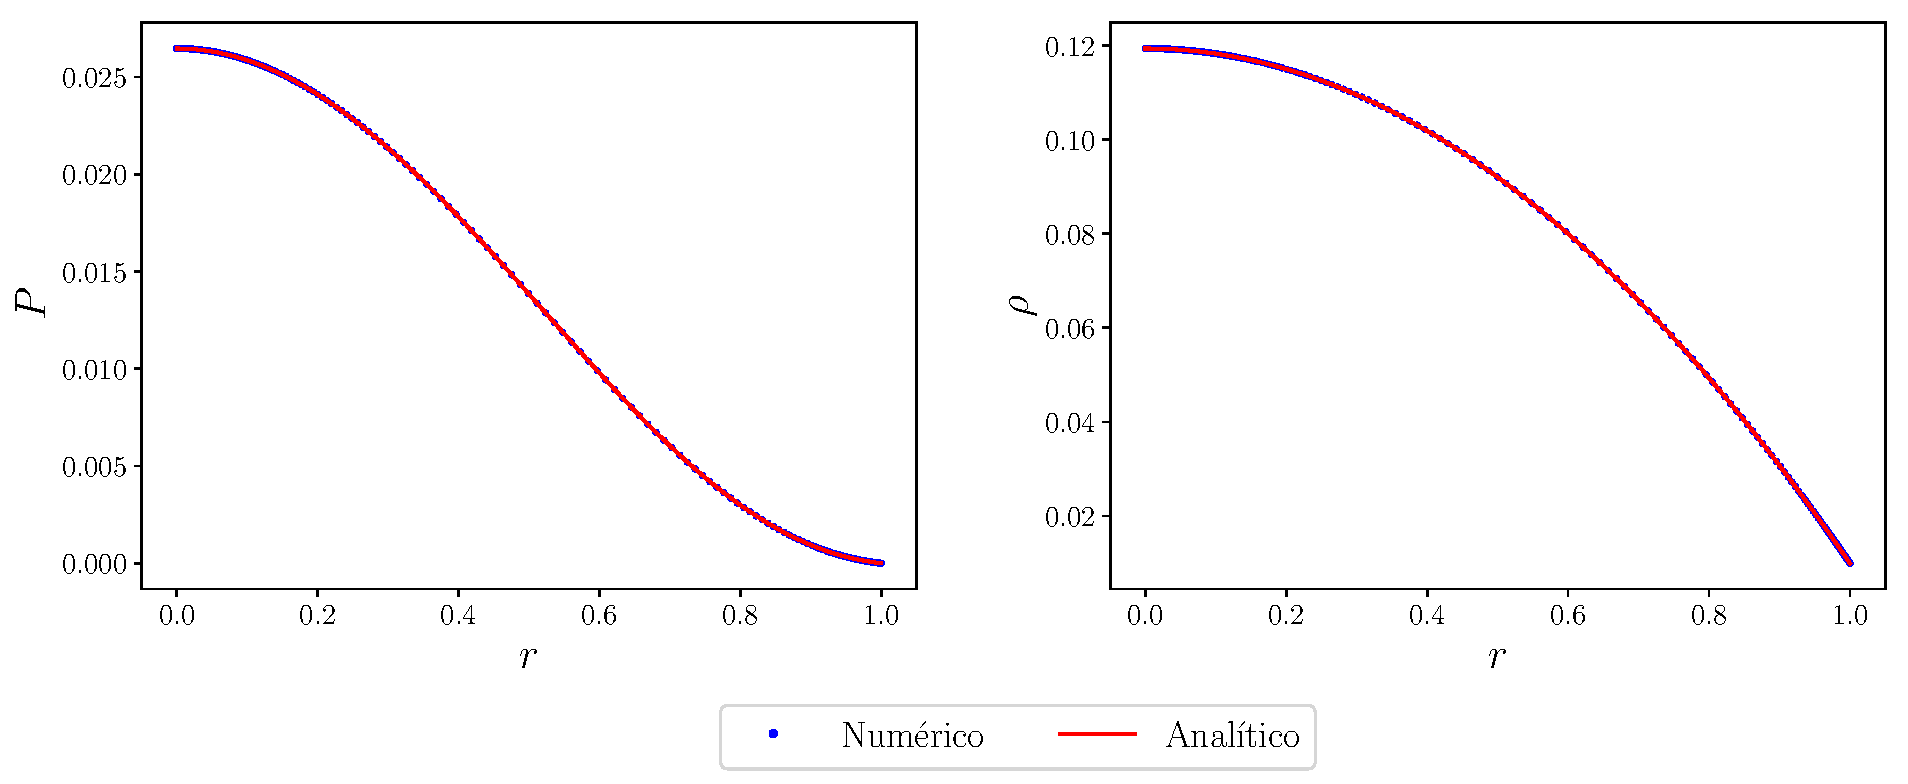
\includegraphics[width=\linewidth]{figures/ProfilesTolmanVIImu45.pdf}
    \caption[Comparación entre una solución exacta y su análogo numérico]{Comparación entre los perfiles de presión y densidad numéricos y analíticos para una compacidad $\mu=0.45$.}
    \label{Exact}
\end{figure}

La convergencia del paso adaptativo usado \eqref{adaptivestep} se puede verificar hallando el error entre la solución exacta y la numérica para distintos valores de $\delta$ ya que $\delta$ maneja la cantidad de pasos que se tomarán por caída de masa y presión (ver Figura \ref{ErrorExact}). 

\begin{figure}%[H]
    \centering
    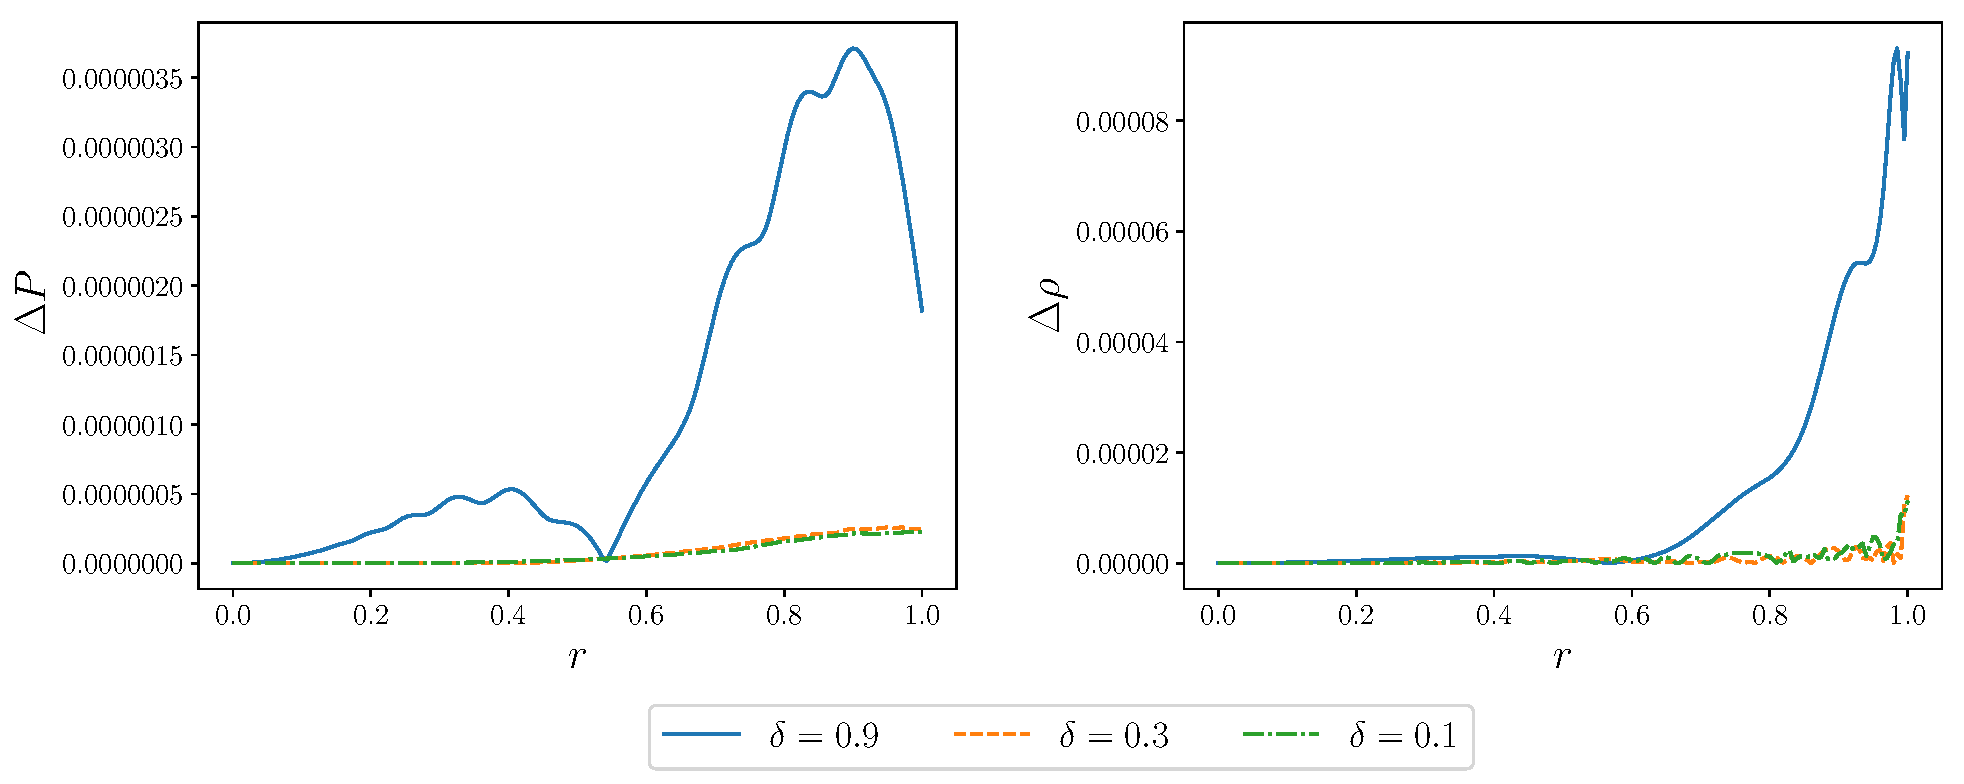
\includegraphics[width=\linewidth]{figures/ErrorTolmanVIImu45.pdf}
    \caption[Error de la solución numérica respecto a la exacta]{Error de la solución numérica como función de $r$ para distintos valores de $\delta$. Para $\delta=0.9$ se obtuvo los errores más grandes, como era de esperarse y converge rápidamente: la diferencia entre usar $\delta=0.3$ y $\delta=0.1$ no es significante.}
    \label{ErrorExact}
\end{figure}


\section{Derivadas numéricas de las variables físicas}\label{NumDer}  

\noindent Para evaluar algunas de las condiciones de aceptabilidad fue necesario hallar derivadas numéricas de un arreglo con respecto a otro. Esto en principio se puede realizar fácilmente usando diferencias finitas, sin embargo la presencia de discontinuidades propias de las EOS y de su interpolación hacen que sea poco práctico usarlas. La alternativa que se encontró fue satisfactoria fue interpolar los arreglos a derivar usando un spline suavizado y hallar la derivada del spline. La librería de Python Scipy\footnote{\url{https://www.scipy.org}} cuenta con una rutina llamada UnivariateSpline\footnote{\url{https://docs.scipy.org/doc/scipy-0.17.0/reference/generated/scipy.interpolate.UnivariateSpline.html}} que permite realizar la interpolación y hallar su derivada fácilmente.
\begin{figure}[H]
    \centering
    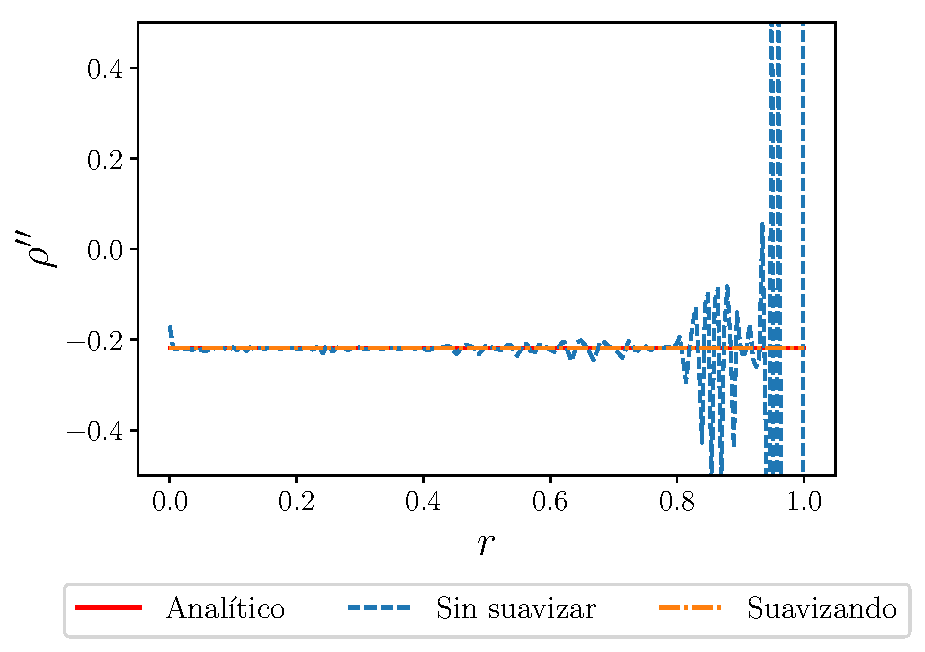
\includegraphics[width=0.7\linewidth]{figures/rhoppTolmanVIImu45.pdf}
    \caption[Comparación entre $\rho^{\prime\prime}$ para una solución exacta y lo obtenido numéricamente]{Comparación de la segunda derivada del perfil de densidad con respecto a $r$ analítica, numérica sin suavizar y suavizada con un factor de suavizamiento de $10^{-5}$, para la solución exacta Tolman VII con $\mu=0.45$. Se aprecia cómo un pequeño factor de suavizamiento es suficiente para obtener una derivada numérica precisa. }
    \label{numericald}
\end{figure}
Como un ejemplo de cómo el hecho de que el spline sea suavizado ayuda a mejorar la derivación numérica, se usó la segunda derivada con respecto a $r$ del perfil de densidad de la solución exacta presentada en la sección anterior y se halló la misma derivada al perfil numérico con la rutina mencionada (ver Figura \ref{numericald}). 
Se puede observar cómo la derivada del spline sin suavizar presenta grandes oscilaciones, que indican un \quotes{overfitting}. Por otro lado al usar un pequeño factor de suavizamiento la cantidad de nodos que se utilizan se reduce y las dos derivadas coinciden.
